\documentclass[a4paper,12pt]{report}

\usepackage{alltt, fancyvrb, url}
\usepackage{graphicx}
\usepackage{subfigure}
\usepackage{wrapfig}
\usepackage{algorithmic}
\usepackage[utf8]{inputenc}
\usepackage{fontenc}
\usepackage{amsmath,stmaryrd,mathtools,algorithm}
\usepackage{amssymb}
\usepackage{float}
\usepackage{hyperref}

% Remove option to use English naming
\usepackage[italian]{cleveref}

% Questo commentalo se vuoi scrivere in inglese.
\usepackage[italian]{babel}

\title{Meta-relazione per\\``Programmazione ad Oggetti''}
 
\author{Giovanni Di Santi}
\date{\today}


\begin{document}
 
\maketitle

\begin{abstract}
Questo documento è una relazione di meta livello, ossia una relazione che spiega come scrivere la relazione.
%
Lo scopo di questo documento è quello di aiutare gli studenti a comprendere quali punti trattare nella loro relazione, ed in che modo farlo, evitando di perdere del tempo prezioso in prolisse discussioni di aspetti marginali tralasciando invece aspetti di maggior rilievo.
%
Per ciascuna delle sezioni del documento sarà fornita una descrizione di ciò che ci si aspetta venga prodotto dal team di sviluppo, assieme ad un elenco (per forza di cose non esaustivo) di elementi che \emph{non} dovrebbero essere inclusi.

Il modello della relazione segue il processo tradizionale di ingegneria del software fase per fase (in maniera ovviamente semplificata).
%
La struttura della relazione non è indicativa ma \textit{obbligatoria}.
%
Gli studenti dovranno produrre un documento che abbia la medesima struttura, non saranno accettati progetti la cui relazione non risponda al requisito suddetto.
%
Lo studente attento dovrebbe sforzarsi di seguire le tappe suggerite in questa relazione anche per l'effettivo sviluppo del progetto: oltre ad una considerevole semplificazione del processo di redazione di questo documento, infatti, il gruppo beneficerà di un processo di sviluppo più solido e collaudato, di tipo top-down.

La meta-relazione verrà fornita corredata di un template \LaTeX{} per coloro che volessero cimentarsi nell'uso.
%
L'uso di \LaTeX{} è vantaggioso per chi ama l'approccio ``what you mean is what you get'', ossia voglia disaccoppiare il contenuto dall'effettivo rendering del documento, accollando al motore \LaTeX{} l'onere di produrre un documento gradevole con la struttura ed il contenuto forniti.
%
Chi non volesse installare l'ambiente di compilazione in locale può valutare l'utilizzo dell'applicazione web \href{https://www.overleaf.com/}{Overleaf}.
%
L'eventuale utilizzo di \LaTeX{} non è fra i requisiti, non è parte del corso di Programmazione ad Oggetti, e non sarà ovviamente valutato. I docenti accetteranno qualunque relazione in formato standard Portable Document Format (pdf), indipendentemente dal software con cui tale documento sarà redatto.
\end{abstract}

\tableofcontents

\chapter{Analisi}

\section{Requisiti}

Il gruppo si pone come obiettivo quello di realizzare un keepass per salvare
in modo sicuro le password. Al momento i keepass desktop più usati sono
\href{https://keepass.info/}{keepass2} e \href{https://keepassxc.org/}{keepassxc}.

\subsubsection{Requisiti funzionali}
\begin{itemize}
  \item Gestione account con possibilità di suddividere gli account in gruppi.
  \item Funzione per generare password e nickname in maniera causale.
  \item Import ed export del database in XML e in un formato simile a KDBX.
  \item Controllo robustezza password al momento dell'inserimento
  \item Salvataggio dei dati in un database locale criptato con algoritmi a scelta
  \item Sezione Statistics che mostra le statistiche relative al proprio database (Es. il numero di account salvati)
\end{itemize}

\subsubsection{Requisiti non funzionali}
\begin{itemize}
	\item bho
\end{itemize}

\section{Analisi e modello del dominio}

In questa sezione si descrive il modello del \textit{dominio 
applicativo}, descrivendo le \textit{entità} in gioco ed i rapporti fra loro.
%
Si possono sollevare eventuali aspetti particolarmente impegnativi, descrivendo perché lo sono, senza inserire idee circa possibili soluzioni, ovvero sull'organizzazione interna del software.
%
Infatti, la fase di analisi va effettuata \textbf{prima} del progetto: né il progetto né il software esistono nel momento in cui si effettua l'analisi.
%
La discussione di aspetti propri del software (ossia, della \textit{soluzione} al problema e non del problema stesso) appartengono alla sfera della progettazione, e vanno discussi successivamente.

È obbligatorio fornire uno schema UML del dominio, che diventerà anche lo scheletro della 
parte ``entity'' del modello dell'applicazione, ovvero degli elementi costitutivi del modello (in ottica MVC - Model View Controller): se l'analisi è ben fatta, dovreste ottenere una gerarchia di concetti che rappresentano le entità che compongono il problema da risolvere.
%
Un'analisi ben svolta \textbf{prima} di cimentarsi con lo sviluppo rappresenta un notevole aiuto per 
le fasi successive: è sufficiente descrivere a parole il dominio, quindi estrarre i sostantivi 
utilizzati, capire il loro ruolo all'interno del problema, le relazioni che intercorrono fra loro, e 
reificarli in interfacce.

\subsection*{Elementi positivi}
\begin{itemize}
	\item Viene descritto accuratamente il modello del dominio.
	\item Alcuni problemi, se non risolubili in assoluto o nel monte ore, vengono dichiarati come problemi che non saranno risolti o sarano risolti in futuro.
	\item Si modella il dominio in forma di UML, descrivendolo appropriatamente.
\end{itemize}

\subsection*{Elementi negativi}
\begin{itemize}
	\item Manca una descrizione a parole del modello del dominio.
	\item Manca una descrizione UML delle entità del dominio e delle relazioni che intercorrono fra loro.
	\item Vengono elencate soluzioni ai problemi, invece della descrizione degli stessi.
	\item Vengono presentati elementi di design, o peggio aspetti implementativi.
	\item Viene mostrato uno schema UML che include elementi implementativi o non utili alla descrizione del dominio, ma volti alla soluzione (non devono vedersi, ad esempio, campi o metodi privati, o cose che non siano equivalenti ad interfacce).
\end{itemize}

\subsection*{Esempio}
GLaDOS dovrà essere in grado di accedere ad un'insieme di camere di test.
%
Tale insieme di camere prende il nome di percorso.
%
Ciascuna camera è composta di challenge successivi.
%
GLaDOS è responsabile di associare a ciascun challenge un insieme di consigli (suggestions) destinati all'utente (subject), dipendenti da possibili eventi.
%
GLaDOS dovrà poter comunicare coi locali cucina per approntare le torte.
%
Le torte potranno essere dolci, oppure semplici promesse di dolci che verranno disattese.

Gli elementi costitutivi il problema sono sintetizzati in \Cref{img:analysis}.

La difficoltà primaria sarà quella di riuscire a correlare lo stato corrente dell'utente e gli eventi in modo tale da generare i corretti suggerimenti.
%
Questo richiederà di mettere in campo appropriate strategie di intelligenza artificiale.

Data la complessità di elaborare consigli via AI senza intervento umano, la prima versione del software fornita prevederà una serie di consigli forniti dall'utente.

Il requisito non funzionale riguardante il consumo energetico richiederà studi specifici sulle performance di GLaDOS che non potranno essere effettuati all'interno del monte ore previsto: tale feature sarà oggetto di futuri lavori.

\chapter{Design}

\section{Architettura}

Per la realizzazione di KeePassJ abbiamo scelto di utilizzare il pattern architetturale
Model-View-Controller (MVC).

TODO: Inserire schema UML MVC.

\section{Design dettagliato}

TODO: Spiegare a grandi linee

\section*{Giovanni Di Santi}

Il mio compito principale del progetto è stato quello di gestire la parte crittografica e
definire la struttura dell'header del database.

\subsection*{CryptoCipher}

\textbf{CryptoCipher} è l'interfaccia che descrive i metodi necessari per effettuare
l'encryption e la decryption di un array di \textt{byte}.\\
Ogni implementazione disponibile di questa interfaccia è un
\href{https://web.cs.ucdavis.edu/~rogaway/papers/ad.pdf}{AEAD Cipher} 
(Authenticated Encryption with Associated Data).\\
Ho scelto questo schema di encryption per rendere il database resistente ad 
attacchi del tipo \textbf{CCA} (Chosen Ciphertext Attack), cifrando il contenuto del
database e autenticando sia il contenuto che l'header (Associated Data).
\begin{figure}[h]
\centering{}
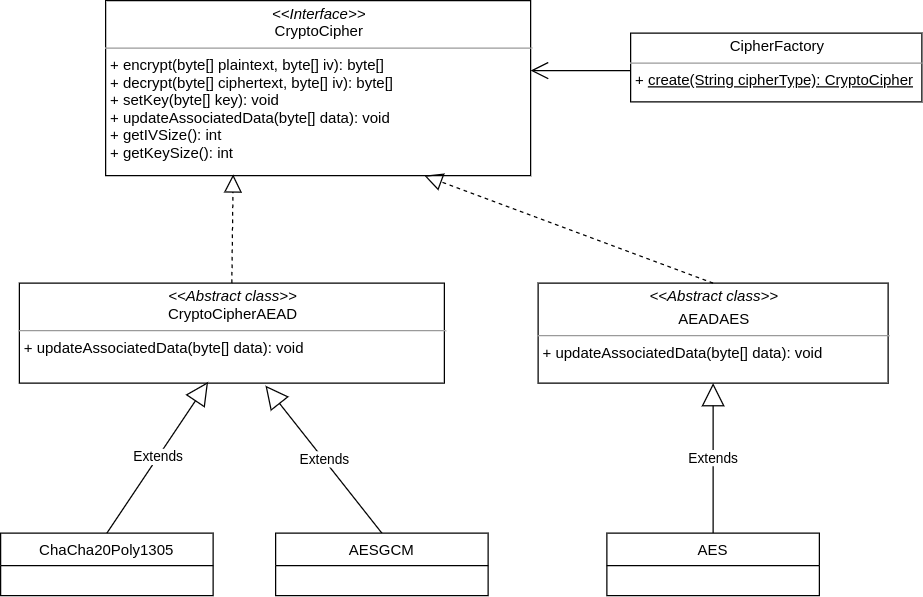
\includegraphics[width=\textwidth]{crypto-cipher}
\caption{rappresentazione UML del pattern factory per creare un CryptoCipher}
\end{figure}
Attualmente i cipher disponibili sono:
\begin{itemize}
  \item \href{https://tools.ietf.org/html/rfc7539}{ChaCha20-Poly1305}.
  \item \href{https://csrc.nist.gov/publications/detail/sp/800-38d/final}{AES-GCM}.
  \item \href{https://tools.ietf.org/html/draft-mcgrew-aead-aes-cbc-hmac-sha2-05}{AES-256-CBC-HMAC-SHA-512}.
\end{itemize}

Esistono due \textt{abstract class} diverse per implementare un \textbf{CryptoCipher},
poiché la costruzione di \textbf{AES} che sarebbe \textt{AES-256-CBC-HMAC-SHA-512} è manuale,
mentre \textbf{ChaCha20-Poly1305} e \textbf{AES-GCM} sono implementate direttamente in openjdk11.
La classe astratta \textbf{AEADAES}, permette di essere estesa per costruire altri
cryptosystem come \textt{AES-192-CBC-HMAC-SHA-384}, tuttavia ho deciso di estendere
solo lo schema più sicuro.\\
Nonostante i dati da cifrare e decifrare sono nella pratica degli \{Input,Output\}Stream,
non ho usato le classi \href{https://docs.oracle.com/en/java/javase/11/docs/api/java.base/javax/crypto/CipherOutputStream.html}{CipherOutputStream}
e \href{https://docs.oracle.com/en/java/javase/11/docs/api/java.base/javax/crypto/CipherInputStream.html}{CipherInputStream}
per:
\begin{itemize}
  \item Rendere più semplice il suo utilizzo.
  \item Facilitare il testing delle varie implementazioni.
\end{itemize}

%Ho usato il design pattern factory per creare un \textbf{CryptoCipher} perché
%quando

\subsection*{KDF}

\textbf{KDF} (Key Derivation Function) è l'interfaccia che descrive i metodi necessari
e opzionali per generare una chiave simmetrica per cifrare/decifrare il database.\\
Gli algoritmi disponibili sono:
\begin{itemize}
  \item Argon2.
  \item Scrypt.
  \item PBKDF2.
\end{itemize}

\begin{figure}[h]
\centering{}
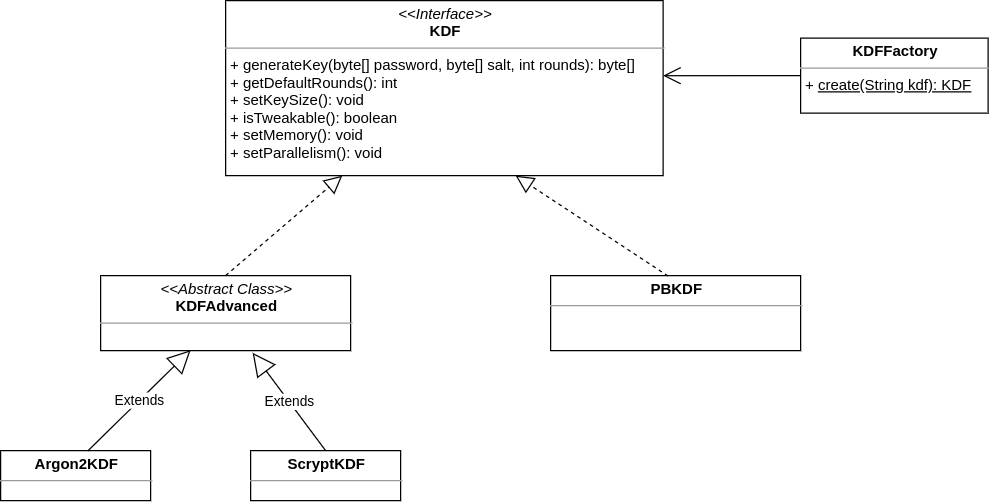
\includegraphics[width=\textwidth]{kdf}
\caption{rappresentazione UML del pattern factory per creare un KDF}
\end{figure}

\textbf{Argon2} e \textbf{Scrypt} estendono \textbf{KDFAdvanced} poiché i loro
algoritmi permettono di definire parametri extra come il paralellismo e la memoria usata
dal KDF. \textbf{PBKDF2} è un vecchio metodo per generare una chiave dalla password e
l'unico parametro configurabile è il numero di round che usa internamente, per questo
ho settato il campo \texttt{tweakable} a falso.

Per capire perché il pattern \texttt{Factory} è usato sia per creare \textbf{KDF}
e \textbf{CryptoCipher} bisogna prima analizzare il parsing dell'header e la relativa
encryption/decryption del database.

\subsection*{KDB}

Per progettare questa parte non ho usato le interfacce perché:
\begin{itemize}
  \item Ho solo una implementazione disponibile.
  \item Sono più flessibile quando devo cambiare la signature di un metodo, senza dover usare un IDE o un LSP per il refactoring.
  \item Principio \href{https://en.wikipedia.org/wiki/You_aren%27t_gonna_need_it}{YAGNI} e \href{https://en.wikipedia.org/wiki/KISS_principle}{KISS}.
\end{itemize}

\textbf{KDBHeader} è la classe che si occupa di:
\begin{itemize}
  \item Parsare l'header (Lettura).
  \item Configurare i vari parametri (Scrittura).
\end{itemize}

\textbf{KDB} è la classe che tramite il \textbf{KDBHeader} si occupa di cifrare/decifrare
dati arbitrari.
Il pattern factory per \textbf{CryptoCipher} e \textbf{KDF} è utile quando in \textbf{KDB}
si effettua l'operazione \texttt{encrypt} e \texttt{decrypt}. I metodi richiedono
a \textbf{KDBHeader} il valore (String) del \texttt{Cipher} e del \texttt{KDF} che viene
passato come parametro di \{Cipher,KDF\}Factory.create() per generare l'oggetto
richiesto.
%Oggetti del tipo \textbf{KDF} e \textbf{CryptoCipher} sono generabili tramite un
%apposita classe \texttt{Factory}. Il vantaggio di usare questo pattern è che quando
%si analizza l'header del database che è diviso in

\begin{figure}[h]
\centering{}
\includegraphics[width=\textwidth]{kdb}
\caption{rappresentazione UML di KDB}
\end{figure}

\chapter{Sviluppo}
\section{Testing automatizzato}

Il testing automatizzato è un requisito di qualunque progetto software che si rispetti, e consente di verificare che non vi siano regressioni nelle funzionalità a fronte di aggiornamenti.
%
Per quanto riguarda questo progetto è considerato sufficiente un test minimale, a patto che sia completamente automatico.
%
Test che richiedono l'intervento da parte dell'utente sono considerati \textit{negativamente} nel computo del punteggio finale.

\subsection*{Elementi positivi}

\begin{itemize}
 \item Si descrivono molto brevemente i componenti che si è deciso di sottoporre a test automatizzato.
 \item Si utilizzano suite specifiche (e.g. JUnit) per il testing automatico.
 \item Se sono stati eseguiti test manuali di rilievo, si elencano descrivendo brevemente la ragione per cui non sono stati automatizzati. Ad esempio, se tutto il team sviluppa e testa su uno stesso sistema operativo e si sono svolti test manuali per verificare, ad esempio, il corretto funzionamento dell'interfaccia grafica o di librerie native su altri sistemi operativi, può avere senso menzionare la cosa.
\end{itemize}

\subsection*{Elementi negativi}
\begin{itemize}
 \item Non si realizza alcun test automatico.
 \item La non presenza di testing viene aggravata dall'adduzione di motivazioni non valide. Ad esempio, si scrive che l'interfaccia grafica non è testata automaticamente perché è \emph{impossibile} farlo\footnote{Testare in modo automatico le interfacce grafiche è possibile (si veda, come esempio, \url{https://github.com/TestFX/TestFX}), semplicemente nel corso non c'è modo e tempo di introdurvi questo livello di complessità. Il fatto che non vi sia stato insegnato come farlo non implica che sia impossibile!}. 
 \item Si descrive un testing di tipo manuale in maniera prolissa.
 \item Si descrivono test effettuati manualmente che sarebbero potuti essere automatizzati, ad esempio scrivendo che si è usata l'applicazione manualmente.
 \item Si descrivono test non presenti nei sorgenti del progetto.
 \item I test, quando eseguiti, falliscono.
\end{itemize}

\section{Metodologia di lavoro}

Ci aspettiamo, leggendo questa sezione, di trovare conferma alla divisione operata nella sezione del design di dettaglio, e di capire come è stato svolto il lavoro di integrazione.
%
\textbf{Andrà realizzata una sotto-sezione separata per ciascuno studente} che identifichi le porzioni di progetto sviluppate, separando quelle svolte in autonomia da quelle sviluppate in collaborazione.
%
Diversamente dalla sezione di design, in questa è consentito elencare package/classi, se lo studente ritiene sia il modo più efficace di convogliare l'informazione.
%
Si ricorda che l'impegno deve giustificare circa 40-50 ore di sviluppo (è normale e fisiologico che approssimativamente la metà del tempo sia impiegata in analisi e progettazione).

\subsection*{Elementi positivi}

\begin{itemize}
	\item Si identifica con precisione il ruolo di ciascuno all'interno del gruppo, ossia su quale parte del progetto ciascuno dei componenti si è concentrato maggiormente.
	\item La divisione dei compiti è equa, ossia non vi sono membri del gruppo che hanno svolto molto più lavoro di altri.
	\item La divisione dei compiti è coerente con quanto descritto nelle parti precedenti della relazione.
	\item La divisione dei compiti è realistica, ossia le dipendenze fra le parti sviluppate sono minime.
	\item Si identifica quale parte del software è stato sviluppato da tutti i componenti insieme.
	\item Si spiega in che modo si sono integrate le parti di codice sviluppate separatamente, evidenziando eventuali problemi. Ad esempio, una strategia è convenire sulle interfacce da usare (ossia, occuparsi insieme di stabilire l'architettura) e quindi procedere indipendentemente allo sviluppo di parti differenti. Una possibile problematica potrebbe essere una dimenticanza in fase di design architetturale che ha costretto ad un cambio e a modifiche in fase di integrazione. Una situazione simile è la norma nell'ingegneria di un sistema software non banale, ed il processo di progettazione top-down con raffinamento successivo è il così detto processo ``a spirale''.
	\item Si descrive in che modo è stato impiegato il DVCS.
\end{itemize}

\subsection*{Elementi negativi}
\begin{itemize}
	\item Non si chiarisce chi ha fatto cosa.
	\item C'è discrepanza fra questa sezione e le sezioni che descrivono il design dettagliato.
	\item Tutto il progetto è stato svolto lavorando insieme invece che assegnando una parte a ciascuno.
	\item Non viene descritta la metodologia di integrazione delle parti sviluppate indipendentemente.
	\item Uso superficiale del DVCS.
\end{itemize}

\section{Note di sviluppo}

Questa sezione, come quella riguardante il design dettagliato va svolta \textbf{singolarmente da ogni membro del gruppo}.

Ciascuno dovrà mettere in evidenza eventuali particolarità del suo metodo di sviluppo, ed in particolare:
\begin{itemize}
	\item \textbf{Elencare} le feature avanzate del linguaggio e dell'ecosistema Java che sono state 
utilizzate. Le feature di interesse sono:
	\begin{itemize}
		\item Progettazione con generici, ad esempio costruzione di nuovi tipi generici, e uso di generici bounded. Uso di classi generiche di libreria non è considerato avanzato.
		\item Uso di lambda expressions
		\item Uso di \texttt{Stream}, di \texttt{Optional} o di altri costrutti funzionali
		\item Uso della reflection
		\item Definizione ed uso di nuove annotazioni
		\item Uso del Java Platform Module System
		\item Uso di parti di libreria non spiegate a lezione (networking, compressione, parsing XML, eccetera...)
		\item Uso di librerie di terze parti (incluso JavaFX): Google Guava, Apache Commons...
		\item Uso di build systems
	\end{itemize}
	Si faccia molta attenzione a non scrivere banalità, elencando qui features di tipo ``core'', come le eccezioni, le enumerazioni, o le inner class: nessuna di queste è considerata avanzata.
	\item Descrivere \textit{molto brevemente} le librerie utilizzate nella propria parte di progetto, se non trattate a lezione (ossia, se librerie di terze parti e/o se componenti del JDK non visti, come le socket). Si ricorda che l'utilizzo di librerie è valutato \emph{positivamente}.
	\item Sviluppo di algoritmi particolarmente interessanti \emph{non forniti da alcuna libreria} (spesso può convenirvi chiedere sul forum se ci sia una libreria per fare una certa cosa, prima di gettarvi a capofitto per scriverla voi stessi).
\end{itemize}
%
In questa sezione è anche bene evidenziare eventuali pezzi di codice ``riadattati'' (o scopiazzati...) da Internet o da altri progetti, pratica che tolleriamo ma che non raccomandiamo.

\subsection*{Elementi positivi}

\begin{itemize}
	\item Si elencano gli aspetti avanzati di linguaggio che sono stati impiegati
	\item Si elencano le librerie che sono state utilizzate
	\item Si descrivono aspetti particolarmente complicati o rilevanti relativi all'implementazione, 
ad esempio, in un'applicazione performance critical, un uso particolarmente avanzato di meccanismi 
di caching, oppure l'implementazione di uno specifico algoritmo.
	\item Se si è utilizzato un particolare algoritmo, se ne cita la fonte originale. Ad esempio, se 
si è usato Mersenne Twister per la generazione dei numeri pseudo-random, si cita \cite{mersenne}.
	\item Si identificano parti di codice prese da altri progetti, dal web, o comunque scritte in forma originale da altre persone. In tal senso, si ricorda che agli ingegneri non è richiesto di re-inventare la ruota continuamente: se si cita debitamente la sorgente è tollerato fare uso di di snippet di codice per risolvere velocemente problemi non banali. Nel caso in cui si usino snippet di codice di qualità discutibile, oltre a menzionarne l'autore originale si invitano gli studenti ad adeguare tali parti di codice agli standard e allo stile del progetto. Contestualmente, si fa presente che è largamente meglio fare uso di una libreria che copiarsi pezzi di codice: qualora vi sia scelta (e tipicamente c'è), si preferisca la prima via.
\end{itemize}

\subsection*{Elementi negativi}
\begin{itemize}
	\item Si elencano feature core del linguaggio invece di quelle segnalate. Esempi di feature 
core da non menzionare sono:
    \begin{itemize}
        \item eccezioni;
        \item classi innestate;
        \item enumerazioni;
        \item interfacce.
    \end{itemize}
	\item Si elencano applicazioni di terze parti (peggio se per usarle occorre licenza, e lo 
studente ne è sprovvisto) che non c'entrano nulla con lo sviluppo, ad esempio:
    \begin{itemize}
        \item Editor di grafica vettoriale come Inkscape o Adobe Illustrator;
        \item Editor di grafica scalare come GIMP o Adobe Photoshop;
        \item Editor di audio come Audacity;
        \item Strumenti di design dell'interfaccia grafica come SceneBuilder: il codice è in ogni caso inteso come sviluppato da voi.
    \end{itemize}
	\item Si descrivono aspetti di scarsa rilevanza, o si scende in dettagli inutili.
	\item Sono presenti parti di codice sviluppate originalmente da altri che non vengono
debitamente segnalate. In tal senso, si ricorda agli studenti che i docenti hanno accesso a tutti i 
progetti degli anni passati, a Stack Overflow, ai principali blog di sviluppatori ed esperti Java (o sedicenti tali), ai blog dedicati allo sviluppo di soluzioni e applicazioni (inclusi blog dedicati ad Android e allo sviluppo di videogame), nonché ai social network. Conseguentemente, è \emph{molto} conveniente \emph{citare} una fonte ed usarla invece di tentare di spacciare per proprio il lavoro di altri.
\end{itemize}

\chapter{Commenti finali}

In quest'ultimo capitolo si tirano le somme del lavoro svolto e si delineano eventuali sviluppi 
futuri.

\textit{Nessuna delle informazioni incluse in questo capitolo verrà utilizzata per formulare la valutazione finale}, a meno che non sia assente o manchino delle sezioni obbligatorie.
%
Al fine di evitare pregiudizi involontari, l'intero capitolo verrà letto dai docenti solo dopo aver formulato la valutazione.

\section{Autovalutazione e lavori futuri}

\textbf{È richiesta una sezione per ciascun membro del gruppo, obbligatoriamente}.
%
Ciascuno dovrà autovalutare il proprio lavoro, elencando i punti di forza e di debolezza in quanto prodotto.
Si dovrà anche cercare di descrivere \emph{in modo quanto più obiettivo possibile} il proprio ruolo all'interno del gruppo.
Si ricorda, a tal proposito, che ciascuno studente è responsabile solo della propria sezione: non è un problema se ci sono opinioni contrastanti, a patto che rispecchino effettivamente l'opinione di chi le scrive.
Nel caso in cui si pensasse di portare avanti il progetto, ad esempio perché effettivamente impiegato, o perché sufficientemente ben riuscito da poter esser usato come dimostrazione di esser capaci progettisti, si descriva brevemente verso che direzione portarlo.

\section{Difficoltà incontrate e commenti per i docenti}

Questa sezione, \textbf{opzionale}, può essere utilizzata per segnalare ai docenti eventuali problemi o difficoltà incontrate nel corso o nello svolgimento del progetto, può essere vista come una seconda possibilità di valutare il corso (dopo quella offerta dalle rilevazioni della didattica) avendo anche conoscenza delle modalità e delle difficoltà collegate all'esame, cosa impossibile da fare usando le valutazioni in aula per ovvie ragioni.
%
È possibile che alcuni dei commenti forniti vengano utilizzati per migliorare il corso in futuro: sebbene non andrà a vostro beneficio, potreste fare un favore ai vostri futuri colleghi.
%
Ovviamente \textit{il contenuto della sezione non impatterà il voto finale}.

\appendix
\chapter{Guida utente}

Capitolo in cui si spiega come utilizzare il software. Nel caso in cui il suo uso sia del tutto 
banale, tale capitolo può essere omesso.
%
A tal riguardo, si fa presente agli studenti che i docenti non hanno mai utilizzato il software 
prima, per cui aspetti che sembrano del tutto banali a chi ha sviluppato l'applicazione possono non 
esserlo per chi la usa per la prima volta.
%
Se, ad esempio, per cominciare una partita con un videogioco è necessario premere la barra 
spaziatrice, o il tasto ``P'', è necessario che gli studenti lo segnalino.

\subsection*{Elementi positivi}

\begin{itemize}
 \item Si istruisce in modo semplice l'utente sull'uso dell'applicazione, eventualmente facendo uso di schermate e descrizioni.
\end{itemize}

\subsection*{Elementi negativi}
\begin{itemize}
 \item Si descrivono in modo eccessivamente minuzioso tutte le caratteristiche, anche minori, del software in oggetto.
 \item Manca una descrizione che consenta ad un utente qualunque di utilizzare almeno le funzionalità primarie dell'applicativo.
\end{itemize}

\bibliographystyle{abbrv}
\bibliography{template}

\end{document}

